%
% File udst2018.tex
%
%% adapted from CONLL 2017 Shared Task on Universal Dependencies for the CoNLL 2018 Shared Task on Universal Dependencies
%% adapted from acl2017.tex for the CoNLL 2017 Shared Task on Universal Dependencies
%% system papers
%%
%% Based on the style files for ACL-2015, with some improvements
%%  taken from the NAACL-2016 style
%% Based on the style files for ACL-2014, which were, in turn,
%% based on ACL-2013, ACL-2012, ACL-2011, ACL-2010, ACL-IJCNLP-2009,
%% EACL-2009, IJCNLP-2008...
%% Based on the style files for EACL 2006 by 
%%e.agirre@ehu.es or Sergi.Balari@uab.es
%% and that of ACL 08 by Joakim Nivre and Noah Smith

\documentclass[11pt,a4paper]{article}
\usepackage[hyperref]{udst2018}
\usepackage{amsmath}
\usepackage{times}
\usepackage{latexsym}
\usepackage{subcaption}
\usepackage{graphicx}
\usepackage{url}


\aclfinalcopy 
\def\aclpaperid{***} %  Enter the Paper ID here for final camera ready copy

%\setlength\titlebox{5cm}
% You can expand the titlebox if you need extra space
% to show all the authors. Please do not make the titlebox
% smaller than 5cm (the original size); we will check this
% in the camera-ready version and ask you to change it back.

\newcommand\BibTeX{B{\sc ib}\TeX}
\newcommand{\yjcomment}[1]{\textcolor{blue}{[$_\mathrm{L}^\mathrm{Y}$#1]}}

\title{Towards Better UD Parsing: Deep Contextualized Word Embeddings, Ensemble, and Treebank Concatenation}

\author{}

\date{}

\begin{document}
\maketitle

\newcommand{\udst}[0]{\emph{CoNLL 2018 UD Shared Task}}

\begin{abstract}
This paper describes our system (HIT-SCIR)
for  CoNLL 2018 shared
task on Universal Dependency parsing.
We base our system on Stanford's winning system for the CoNLL 2017 shared task
and made two effective extensions: ensembling
parsers trained with different initialization
and incorporating deep contextualized
word embeddings into both the POS
tagger and parser.
We also explore different ways of concatenating treebanks
and it leads further improvements.
Experimental results on the development data
show the effectiveness of our methods.
In the evaluation on the test data,
our system was ranked first according to LAS (75.84\%)
and outperformed the secondly ranked system by 2.56\%.

\end{abstract}

\section{Introduction}

In this paper, we describe our system (HIT-SCIR) submitted to CoNLL 2018 shared
task on Universal Dependency parsing \cite{udst:overview}.
We base our system on Stanford's winning system \citep[\S\ref{sec:biaffine}]{dozat-qi-manning:2017:K17-3}
for the CoNLL 2017 shared task \cite{udst:overview2017}.
\citet{DBLP:journals/corr/DozatM16} and
its extension \cite{dozat-qi-manning:2017:K17-3} have
show very competitive performance in previous parsing works \cite{ma-hovy:2017:I17-1,shi-huang-lee:2017:EMNLP2017,N18-1088,DBLP:journals/corr/abs-1805-01087}.
In this paper, we would like to know can we further improve
their POS tagger and parser with cheap and universal solution.

In our system, we make two noteworthy extensions to their parser and tagger,
which includes
\begin{itemize}
	\item Incorporating the deep contextualized word embeddings \cite[ELMo]{N18-1202} into the word representaton (\S\ref{sec:elmo}).
	\item Ensembling parsers trained with different initialization (\S\ref{sec:ens}).
\end{itemize}

In the shared task, multiple treebanks of different domains are provided for some languages.
There are also treebanks which are of the same language families.
Letting these treebanks help each other has been shown an effective way to improve parsing performance
in last year's shared tasks \citep{che-EtAl:2017:K17-3,shi-EtAl:2017:K17-3,bjorkelund-EtAl:2017:K17-3}.
In our system, we apply the simple concatenation to the treebanks that are potentially
helpful to each other
and explore different ways of concatenation to improve the parser's performance (\S\ref{sec:comb}).

In dealing with the small languages and low-resource languages (\S\ref{sec:low}),
we adopt the word embedding transfer idea 
in the cross-lingual dependency parsing \cite{guo-EtAl:2015:ACL-IJCNLP2}
and use the bilingual word vectors transformation technique \cite{DBLP:journals/corr/SmithTHH17}
to map \textit{fasttext} word embeddings \cite{DBLP:journals/corr/BojanowskiGJM16}
of the source rich-resource language and target low-resource language
into the same space and transfer the parser trained on the source language into the target language.

We conduct experiments on the development set to study
the effects of ELMo, parser ensemble, and treebank concatenation.
Experimental results show that these techniques substantially improve the parsing performance.
Using these techniques, our system achieved an averaged LAS of 75.84 on the official test set
and was ranked the first according to LAS \cite{udst:overview}.
This result outperforms the seondly ranked by 2.56\%.

\section{\citet{dozat-qi-manning:2017:K17-3}}\label{sec:biaffine}

We based our system on the tagger and parser of \citet{dozat-qi-manning:2017:K17-3}.
The core idea of the tagger and parser
is using a LSTM network to produce the vector representation
for each word and then predict POS tags and dependency relations
using the representation.
For the tagger whose input is the word alone,
this representation is calculated as
\begin{align*}
\mathbf{r}_i & =  \text{BiLSTM}(\mathbf{r}_0, (\mathbf{v}_1^{(word)}, ..., \mathbf{x}_n^{(word)}))_i \\
\mathbf{h}_i, \mathbf{c}_i & = \text{split}(\mathbf{r}_i),
\end{align*}
where $\mathbf{v}_i^{(word)}$ is the word embeddings.
After getting $\mathbf{h}_i$,
the scores of tags are calculated as
\begin{align*}
\mathbf{h}_i^{(pos)} & = \text{MLP}^{(pos)} (\mathbf{h}_i) \\
\mathbf{s}_i^{(pos)} & = W \cdot \mathbf{h}_i^{(pos)} + \mathbf{b}^{(pos)}
\end{align*}
where each element in $\mathbf{s}_i^{(pos)}$ represents the possibility
that $i$-th word is assigned with corresponding tag.

For the parser whose inputs are the word and POS tag,
such representation is calculated as
\begin{align*}
\mathbf{x}_i & =  \mathbf{v}_i^{(word)} \oplus \mathbf{v}_i^{(tag)} \\
\mathbf{r}_i & =  \text{BiLSTM}(\mathbf{r}_0, (\mathbf{x}_1, ..., \mathbf{x}_n))_i \\
\mathbf{h}_i, \mathbf{c}_i & = \text{split}(\mathbf{r}_i)\text{.}
\end{align*}
And a pair of representations are fed into a biaffine classifier
to predict if there is a dependency arc between these two words.
The scores over all head words are calculated as
\begin{align*}
\mathbf{s}_i^{(rel)} & = \mathbf{h}^{T(rel-head)}_{y^{‘(arc)}} \mathbf{U}^{(rel)} \mathbf{h}_i^{(rel-dep)} \\
& + W^{(rel)} (\mathbf{h}_i^{(rel-dep)} \oplus \mathbf{h}^{T(rel-head)}_{y^{‘(arc)}}) \\
& + \mathbf{b}^{(rel)}
\end{align*}

For both the biaffine tagger and parser, 
the word embedding $\mathbf{v}_i^{(word)}$ is obtained by summarizing 
a fine-tuned token embedding $\mathbf{w}_i$, a fixed word2vec embedding $\mathbf{p}_i$, and a LSTM-encoded
character representation $\mathbf{\hat{v}}_i$ as
\[
\mathbf{v}_i^{(word)} = \mathbf{w}_i + \mathbf{p}_i + \mathbf{\hat{v}}_i
\]

\section{Deep Contextualized Word Embeddings}\label{sec:elmo}

Deep contextualized word embeddings \citep[ELMo]{N18-1202}
has shown to
be very effective on a range of syntactic and semantic tasks
and it's straightforward to achieve by
using a LSTM network to encode words in a sentence
and training the LSTM network with language modeling objective
on large-scale raw text.
More specifically, the $\mathbf{ELMo}_i$ is computed
by first computing the hidden representation $\mathbf{h}_i^{(LM)}$ as
\begin{align*}
\mathbf{r}_i^{(LM)} & =  \text{BiLSTM}^{(LM)}(\mathbf{r}_0^{(LM)}, (\mathbf{\tilde{v}}_1, ..., \mathbf{\tilde{v}}_n))_i \\
\mathbf{h}_i^{(LM)}, \mathbf{c}_i^{(LM)} & = \text{split}(\mathbf{r}_i^{(LM)})\text{,}
\end{align*}
where $\mathbf{\tilde{v}}_i$ is the output of a CNN over characters,
then attentively summarizing and scaling different layers of  $\mathbf{h}_{i, j}^{(LM)}$
with $s_j$ and $\gamma$
as
\[
\mathbf{ELMo}_i = \gamma \sum_{j=0}^L s_j \mathbf{h}_{i, j}^{(LM)},
\]
where $L$ is the number of layers and $\mathbf{h}_{i, 0}^{(LM)}$ is identical to $\mathbf{\tilde{v}}_i$.
In our system, we follow \citet{N18-1202} and use a two-layer bidirectional LSTM as our $\text{BiLSTM}^{(LM)}$.

In this paper, we study the usage of ELMo for improving both
the tagger and parser and make several simplifications.
Different from \citet{N18-1202}, we treat the output of ELMo as a fixed representation
and do not tune its parameters during tagger and parser training.
Thus, we cancel the layer-wise attention scores $s_j$ and the scaling factor $\gamma$.
As \citet{N18-1202} pointed, the second layer of $\text{BiLSTM}^{(LM)}$ mainly captures the semantic
information, and we care more about its syntactic part (i.e. the first layer of $\text{BiLSTM}^{(LM)}$).
In our system, we only use $\mathbf{h}_{i, 0}^{(LM)}$ and $\mathbf{h}_{i, 1}^{(LM)}$ for $\mathbf{ELMo}_i$
which means
\[
\mathbf{ELMo}_i = \mathbf{h}_{i, 0}^{(LM)}  +  \mathbf{h}_{i, 1}^{(LM)}.
\]

After getting $\mathbf{ELMo}_i$, we project it
to the same dimension as $\mathbf{v}_i^{(word)}$ and
use it as an additional word embeddings.
The calculation of $\mathbf{v}_i^{(word)}$ becomes
\[
\mathbf{v}_i^{(word)} = \mathbf{w}_i + \mathbf{p}_i + \mathbf{\hat{v}}_i + W^{(ELMo)} \cdot \mathbf{ELMo}_i
\]
for both the tagger and parser.
We need to note that training the tagger and parser includes $W^{(ELMo)}$.
To avoid overfitting, we impose a dropout function on projected vector
$W^{(ELMo)} \cdot \mathbf{ELMo}_i$
during training.

We use the same hyperparameter settings as \citet{N18-1202} for $\text{BiLSTM}^{(LM)}$
and the character CNN.
We train their parameters
as training a bidirectional language model
on a randomly sampled subset of raw text released by the shared task.
More specifically, for each language, we randomly sample 20 million words.
The training of ELMo on one language takes roughly 3 days on an NVIDIA P100 GPU.

\section{Parser Ensemble}\label{sec:ens}

%We seek to use ensemble to improve the performance.
According to \citet{reimers-gurevych:2017:EMNLP2017}, neural network training can
be sensitive to initialization and
\citet{DBLP:journals/corr/abs-1805-11224}  shows that ensemble
neural network trained with different initialization
leads to performance improvements.
We follow their works and train three parsers with different initialization,
then ensemble these parsers by averaging their output scores as 
$\mathbf{s}_i^{(rel)} = \frac{1}{3} \sum_{i=1}^{3} \mathbf{s}_i^{(i, rel)}$.

\section{Treebank Concatenation}\label{sec:comb}

For 15 out of the 58 languages in the shared task,
multiple treebanks from different domains are provided.
There are also treebanks that comes from the same language families.
Taking the advantages of the relation between treebanks has been shown 
a promising direction in both the research community \cite{TACL892,guo-EtAl:2015:ACL-IJCNLP2,C16-1002}
and in the CoNLL 2017 shared task \cite{che-EtAl:2017:K17-3,bjorkelund-EtAl:2017:K17-3,shi-EtAl:2017:K17-3}.
In our system, we adopt the treebank concatenation technique as \cite{TACL892}
but limit that only a group of treebanks from the same language (\textit{cross-domain concatenation})
or a pair of treebanks that are typologically or geographically correlated (\textit{cross-lingual concatenation})
is concatenated.

In our system, we tried cross-domain concatenation on
\textit{nl}, \textit{sv}, \textit{ko}, \textit{it}, \textit{en}, \textit{fr},
\textit{gl}, \textit{la}, \textit{ru}, and \textit{sl}.
We also tried cross-lingual concatenation on \textit{ug-tr}, \textit{uk-ru}, \textit{ga-en},
and \textit{sme-fi} following \cite{che-EtAl:2017:K17-3}.
However, due to the variance in vocabulary, grammatical genre, and even annotation, 
treebank concatenation does not guarantee to improve the model's performance.
We decide the usage of concatenation by examining their development set performance.
For some small treebanks which do not have development set, whether using treebank concatenation
is decided through 5-fold cross validation.\footnote{We use \textit{udpipe} \citep{udpipe} 
	for the experiments of these part
	because we consider the effect of treebank concatenation as
	being irrelevant to the parser architecture
	and \textit{udpipe} has the speed advantage in both training and testing.}
We show the experimental results of treebank concatenation
in Section \ref{sec:treebank-concat}.

%
%\subsection{Cross-Domain Concatenation}
%
%We test the performance of treebank concatenation.


%Based on the results in Table \ref{tbl:confuse-mat} and Table \ref{tbl:confuse-mat2},
%we apply cross-domain concatenation to the treebank where concatenation
%improves either the development or cross validation performance.
%
%\subsection{Cross-Lingual Concatenation}
%

\section{Low Resources Languages}\label{sec:low}
\begin{table}[t]
	\centering
	\small
	\begin{tabular}{r|cccccccc}
		target & br & fo & hy & kk & bxr & kmr & hsb & th \\
		\hline
		source & ga & no & et & tr &  hi & fa & pl & zh \\
	\end{tabular}
\caption{Cross-lingual transfer settings for low-resource target languages.}\label{tbl:low-res-trans}
\end{table}

In the shared task, 5 languages are presented with training set of less than 50 sentences.
4 languages don't even have any training data.
It's difficult to train reasonable parser on these low-resource languages
We deal with these treebanks by adopting the word embedding transfer idea 
of \citet{guo-EtAl:2015:ACL-IJCNLP2}.
We transfer the word embeddings of the rich-resource language
to the space of low-resource language using the bilingual word vectors transformation technique
\cite{DBLP:journals/corr/SmithTHH17}
and trained a parser using the source treebank
with only pretrained word embeddings on the transformed space
as $\mathbf{v}_i^{(word)} = \mathbf{p}_i$.
The transformation matrix is automatically learned on the \textit{fasttext} word embedding
using the same tokens between two languages (like punctuations).

Table \ref{tbl:low-res-trans} shows our source languages for the target low-resource languages.
For the treebank with a few training data, its  source language is decided by
testing the source parser's performance on the training data.
For the treebank without any training data, we choose the source language according to their language family.

\textit{Naija} presents an exception for our method since it doesn't have \textit{fasttext}
word embeddings and embedding transformation is infeasible.
Since it's a dialect of English, we use the full pipeline of \textit{en\_ewt} for \textit{pcm\_nsc}.
\begin{figure*}[t]
	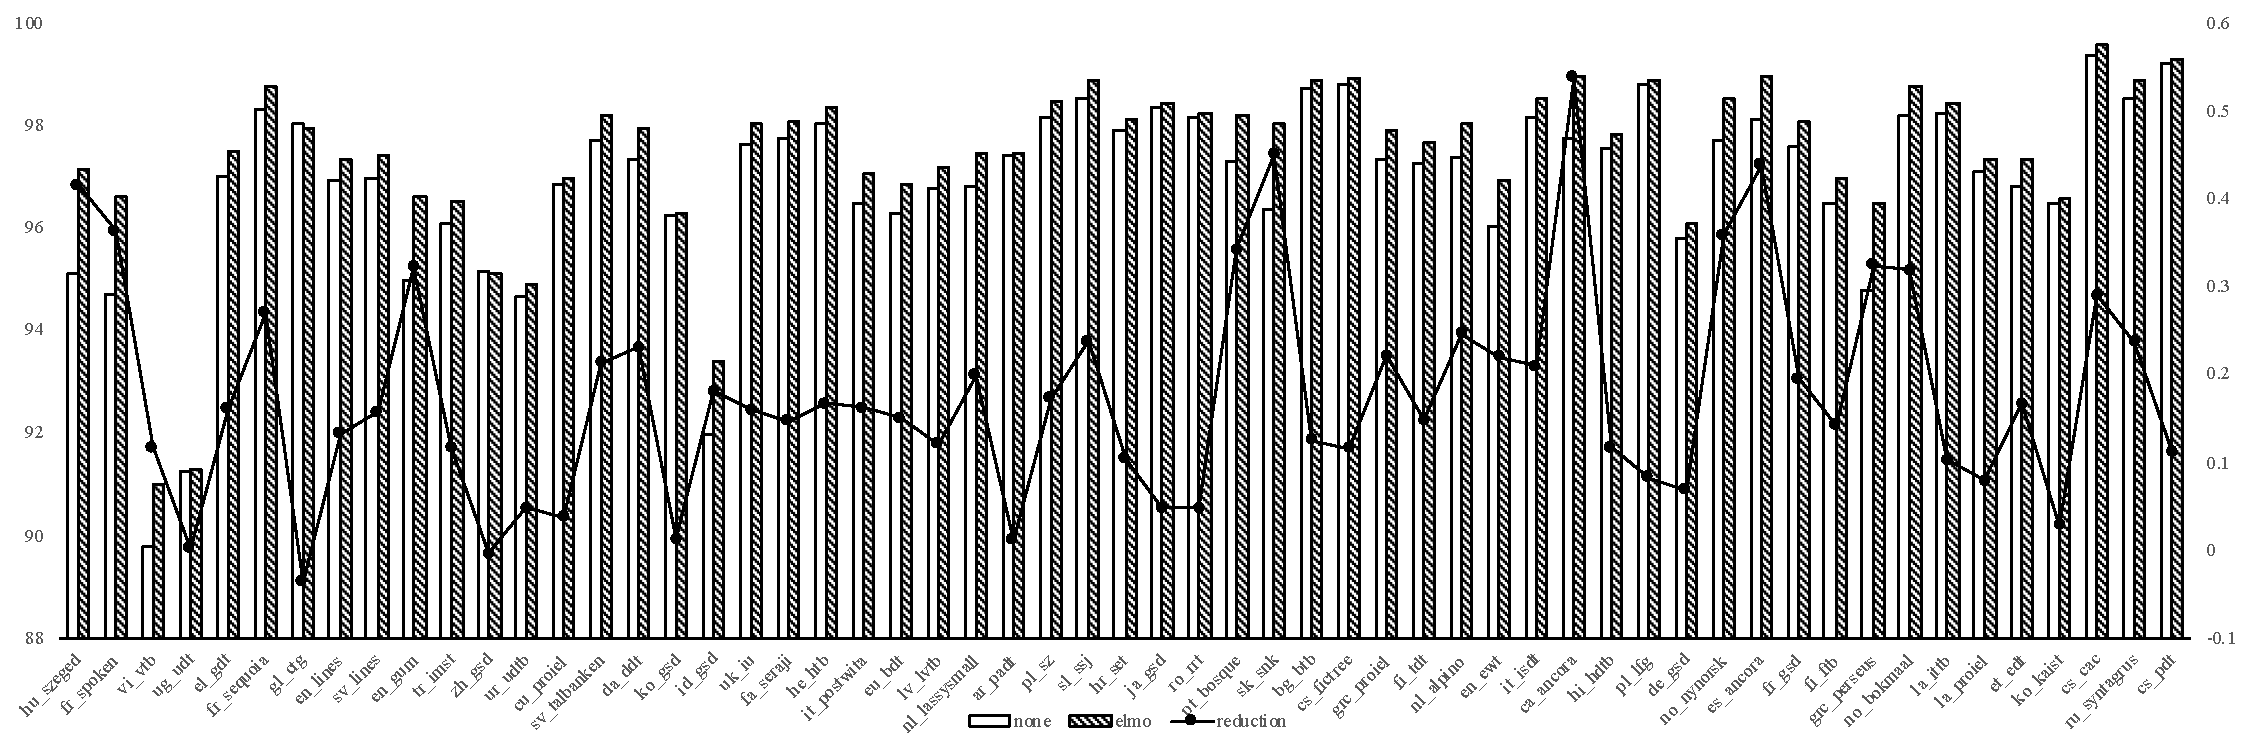
\includegraphics[width=\textwidth]{effects_elmo_tagger}
	\caption{The effects of ELMo on POS tagging.
		Treebanks are sorted according to the number of training sentences from left to right.}\label{fig:elmo-effect-pos}
\end{figure*}
\begin{figure*}[t]
	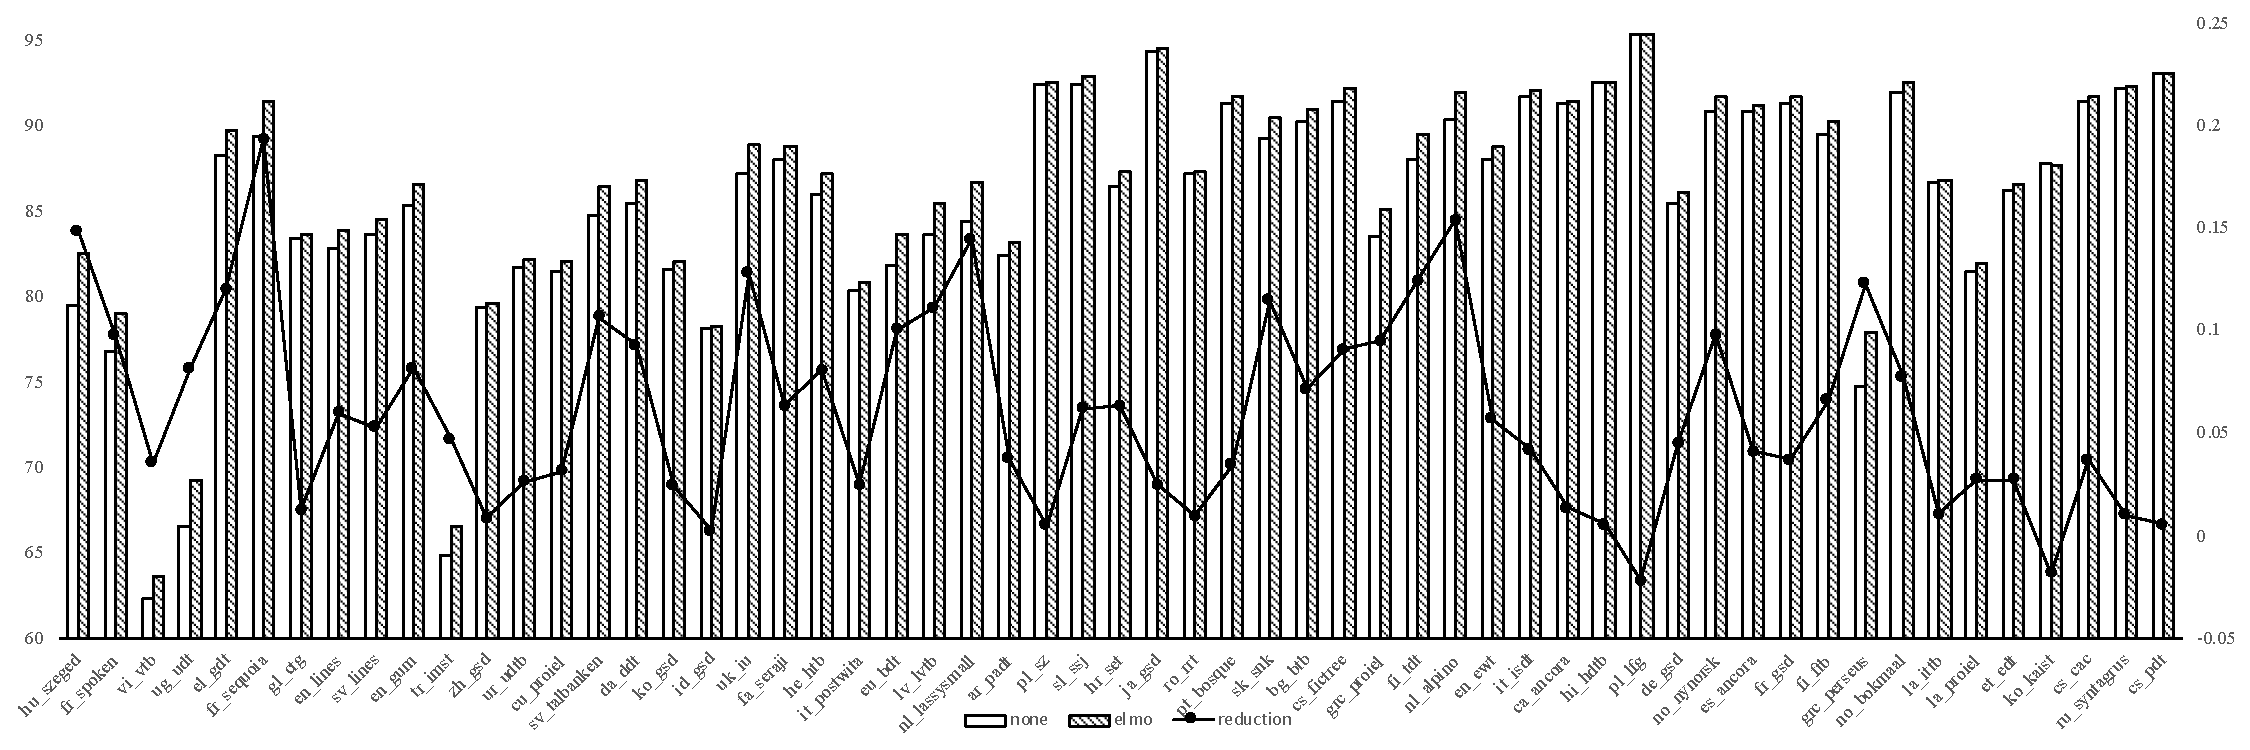
\includegraphics[width=\textwidth]{effects_elmo_parser}
	\caption{The effects of ELMo on parsing.
		Treebanks are sorted according to the number of training sentences from left to right.}\label{fig:elmo-effect-par}
\end{figure*}

\section{Preprocessing}
Besides improving the tagging and parsing performance,
we also consider the preprocessing as an important factor to
the final performance.

\subsection{Sentence Segmentation}
For some treebanks, sentence segmentation can be problematic
since there is no explicitly sentence delimiters.
\citet{delhoneux-EtAl:2017:K17-3} presented a joint tokenization and
sentence segmentation model\footnote{noted as Uppsala segmentor henceforth.}
that outperformed the baseline model in last year's shared task \cite{udst:overview2017}.
We select a set of treebanks whose \textit{udpipe} sentence segmentation F-scores
are lower than 95 on the development set and use Uppsala segmentor instead.\footnote{
	We use Uppsala segmentor for \textit{it\_postwita}, \textit{got\_proiel}, \textit{la\_poroiel}, \textit{cu\_proiel},
	\textit{grc\_proiel}, \textit{sl\_ssj}, \textit{nl\_lassysmall}, \textit{fi\_tdt}, \textit{pt\_bosque}, \textit{da\_ddt}, \textit{id\_gsd},
	\textit{el\_gdt}, and \textit{et\_edt}.}
Using the Uppsala segmentor leads to an improvement of 7.67 F-score in these treebanks over \textit{udpipe} baseline.

\subsection{Tokenization for Chinese, Japanese, and Vietnamese}

Tokenization is non-trivial for languages 
which do not have explicit word boundary markers, like Chinese, Japanese, and Vietnamese.
We develop our own tokenizer for these three languages.
Following \citet{che-EtAl:2017:K17-3} and \citet{10.1007/978-3-319-69005-6_6}, we model the tokenization as labeling the
word boundary tag on character and 
use features derived from large-scale unlabeled data to further improve the performance.\footnote{For Vietnamese where whitespaces occur both inter- and intra-words, we treat the whitespace-separated token as a character.}
In addition to the pointwise mutual information (PMI), we also incorporate
the character ELMO into our tokenizer.
These techniques lead to the best tokenization performance on all the related treebanks
and the average improvement over \textit{udpipe} baseline is 7.5 in tokenization F-score.\footnote{\textit{ja\_gsd}, \textit{ja\_modern}, \textit{vi\_vtb}, and \textit{zh\_gsd}.}

\subsection{Preprocessing for Thai}

Thai language presents unique challenge in the preprocessing.
Our survey on the Thai Wikipedia indicates that there is no explicit sentence delimiter for Thai language
and obtaining Thai words requires tokenization.
To this remedy, we use space as sentence delimiter and
use the lexicon-based word segmentation -- forward maximum matching algorithm
for Thai tokenization.
Our lexicon is derived from the \textit{fasttext} word embeddings.

\section{Results}
\begin{figure*}[t]
	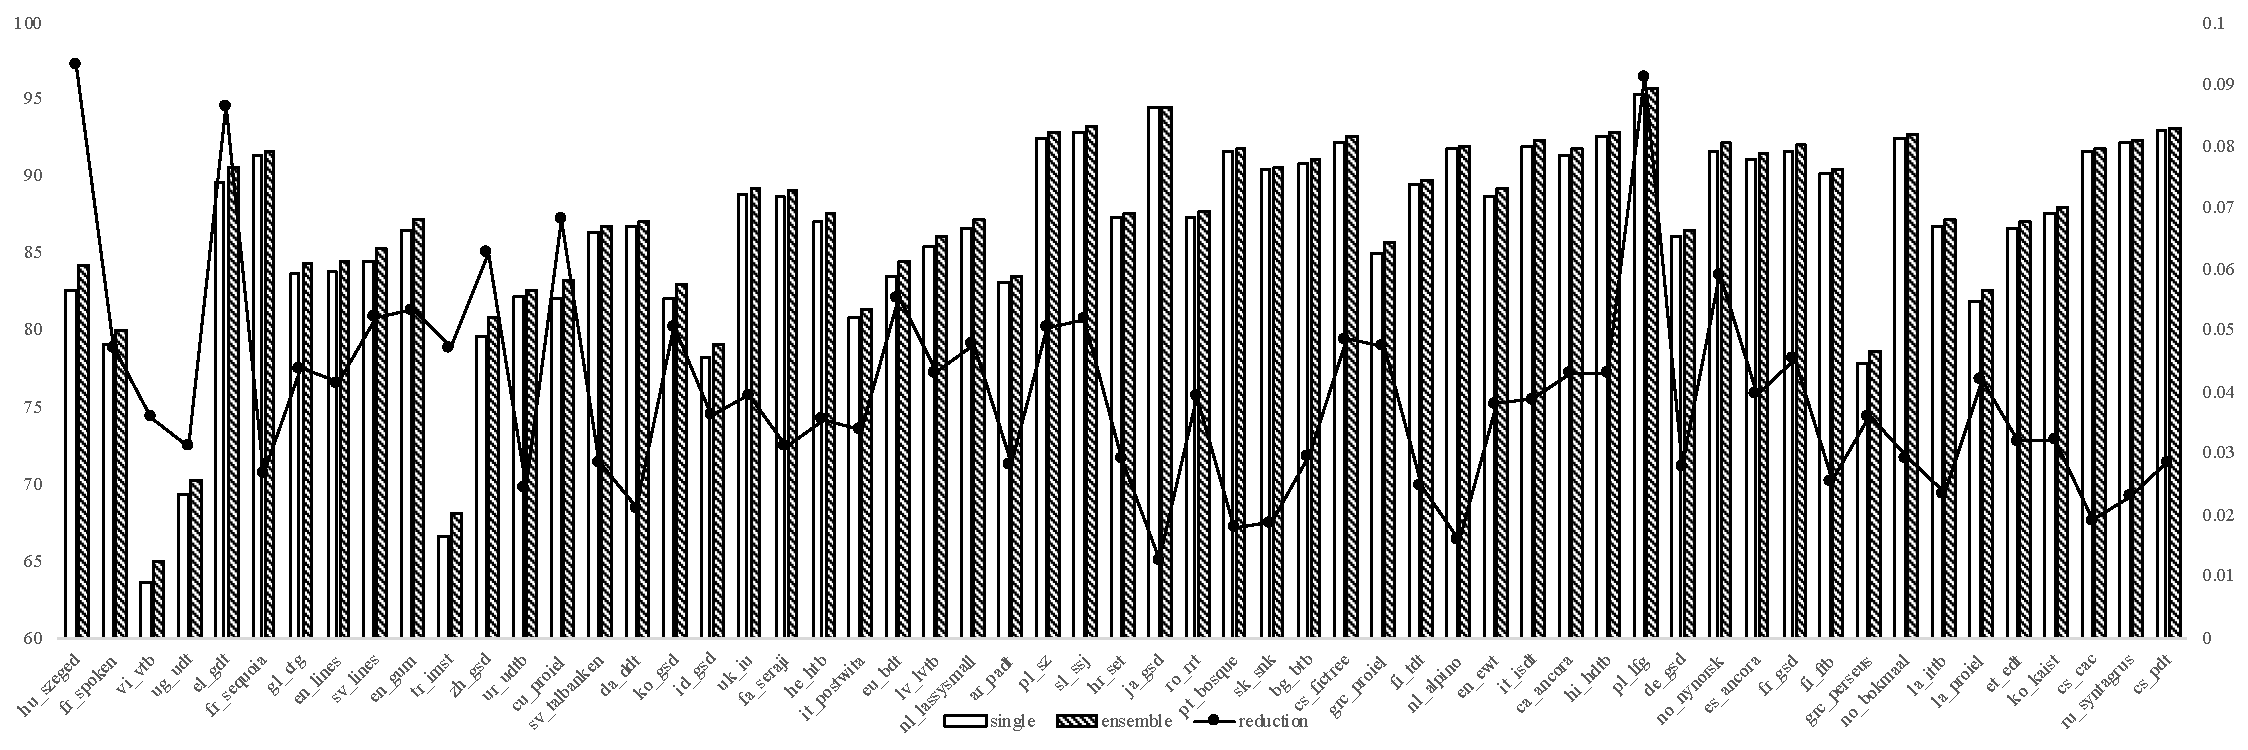
\includegraphics[width=\textwidth]{effects_elmo_ensemble}
	\caption{The effects of ensemble on parsing.
		Treebanks are sorted according to the number of training sentences from left to right.}\label{fig:elmo-effect-ens}
\end{figure*}

%\subsection{Settings}
%
%\paragraph{Pretrained Word Embeddings.}
%For large treebank, we use the 100-dimensional word embeddings as $\mathbf{p}_i$
%in both the biaffine tagger and parser.

\subsection{Effects of ELMo}

We study the effect of ELMo on the large treebanks and report
the results of singe tagger and parser with and without ELMo.
Figure \ref{fig:elmo-effect-pos} shows the tagger results on the development set
and Figure \ref{fig:elmo-effect-par} 
shows the parser results.
Using ELMo in the tagger leads to a macro-averaged improvement of 0.56\% in UPOS
and the macro-averaged error reduction is 17.83\%.
and using ELMo in the parser leads to a macro-averaged improvement 
of 0.84\% in LAS and
the macro-averaged error reduction is 7.88\%.

ELMo improves the tagging performance almost on every treebank,
except for \textit{zh\_gsd} and \textit{gl\_ctg}.
Similar trends are witnessed in the parsing experiments with \textit{ko\_kaist}
and \textit{pl\_lfg} being the only treebanks that ELMo slightly worsens the performance.

We also study the relative improvements against the size of the treebank.
However, no clear relation is revealed between the treebank size and the gains using ELMo.
\begin{table*}[t]
	\centering
	\small
	\setlength{\tabcolsep}{5pt}
	\begin{tabular}{rcc || rcc || rcc || rcc}
		%	\hline
		\textit{nl} & apino & lassysmall & \textit{sv} & lines & talbanken & \textit{ko} & gsd & kaist & \textit{it} & isdt & postwita \\
		\# train & 12.2 & 5.8 & \# train & 2.7 & 4.3 & \# train & 4.4 & 23.0 & \# train & 13.1 & 5.4 \\
		\hline
		apino & 91.87 & & lines & 84.64 & & gsd & 82.05 & & isdt & \textbf{92.01} & \\
		lassysmall & & 86.82 & talbanken & & 86.39 & kaist & & \textbf{87.83} & postwita & & 80.79 \\
		\hline
		concat. & \textbf{92.08} & \textbf{89.34} & concat. & \textbf{85.76} & \textbf{86.77} & concat. & \textbf{83.73} & 87.61 & concat.& 91.80 & \textbf{82.54} \\
		%	\hline
		\vspace*{0.5em}
	\end{tabular}
	\begin{tabular}{rccc || rccc}
		\textit{en} & ewt & gum & lines & \textit{fr} & gsd & sequoia & spoken \\
		\# train & 12.5 & 2.9 & 2.7 & \# train & 14.6 & 2.2 & 1.2\\
		\hline
		ewt & \textbf{88.75} & & & gsd & \textbf{91.64} & & \\
		gum & & \textbf{86.52} & & sequoia & & \textbf{91.44} & \\
		lines & & & 83.86 & spoken & & & 79.06 \\
		\hline
		concat. & 88.74 & 85.65 & \textbf{85.30} & concat. & 91.44 & 90.51 & \textbf{81.99} \\
	\end{tabular}
	\caption{The developement performance with cross-domain concatenation for languages which has multiple treebanks.
		\textit{\# train} shows the number of training sentences in the treebank.
		We opt out \textit{cs}, \textit{fi}, and \textit{pl} because all the treebanks of these languages are relatively large (\# train $>$ 10K).}\label{tbl:confuse-mat}
\end{table*}

\subsection{Effects of Ensemble}

We also test the effect of ensemble and show
the results in Figure \ref{fig:elmo-effect-ens}.
Parser ensemble leads to an averaged improvement of 0.55\% in LAS
and the averaged error reduction is 4.0\%.
These results indicate that ensemble is a effective way of
improving the parsing performance.

\subsection{Effects of Treebank Concatenation}\label{sec:treebank-concat}
As mentioned in Section \ref{sec:comb},
we study the effects of both the \textit{cross-domain concatenation} and \textit{cross-lingual concatenation}.
\paragraph{Cross-Domain Concatenation.}


\begin{table*}[t]
	\centering
	\small
	\begin{tabular}{rc || rc || rc || rc || rc}
		\textit{gl} & treegal & \textit{la} & perseus & \textit{no} & nynorsklia & \textit{ru} & taiga & \textit{sl} & sst \\
		\# train & 0.6 & \# train & 1.3 & \# train & 0.3 & \# train & 0.9 & \# train & 2.1 \\
		\hline
		treegal & \textbf{66.71} & perseus & 44.05 & nynorsklia & 51.05 & taiga & 54.70 & sst & 55.15 \\
		+ctg & 56.73 & +proiel & \textbf{50.78} & +nynorsk & \textbf{58.49} & +syntagrus & \textbf{60.75} & +ssj & \textbf{59.52} \\
	\end{tabular}
	\caption{The 5-fold cross validation results for the cross-domain concatenation for treebank which doesn't have development set.}\label{tbl:confuse-mat2}
\end{table*}

For the treebanks which have development set, the development performances
are shown in Table \ref{tbl:confuse-mat}.
Numbers of sentences in the training set are also shown in this table.
The general trend is that for the treebank with small training set,
cross-domain concatenation achieves better performance.
While for those with large training set, concatenation doesn't improve
the performance or even worsen the results.

For the small treebanks which do not have development set,
the 5 fold cross validation results are shown in Table \ref{tbl:confuse-mat2}
in which concatenation improves most of the treebanks except for \textit{gl\_treegal}.

\paragraph{Cross-Lingual Concatenation.}
\begin{table*}[t]
	\centering
	\small
	%\setlength{\tabcolsep}{5pt}
	\begin{tabular}{rc || rc || rc || rc}
		& ug\_udt  &  & uk\_iu & & ga\_idt & & sme\_giella \\
		\hline
		ug\_udt & \textbf{69.27} & uk\_iu & 88.84 & ga\_idt & \textbf{62.84} & sme\_giella & \textbf{66.33}\\
		+tr\_imst & 19.27 & +ru\_syntagus & \textbf{90.74} & +en\_ewt &51.00 & +fi\_ftb & 59.86\\
	\end{tabular}
	\caption{Cross-lingual concatenation results. 
		The results for \textit{ug\_udt} and \textit{uk\_iu} are obtained on the development set.
		The results for \textit{ga\_idt} and \textit{sme\_giella} are obtained with \textit{udpipe} by 5-fold cross validation.}\label{tbl:cross-ling-concat}
\end{table*}

The experimental results of cross-lingual concatenation are shown in Table \ref{tbl:cross-ling-concat}.
Unfortunately, concatenating treebanks from different languages only
achieves improved performance on \textit{uk\_iu}.
This results also indicate that in cross lingual parsing,
sophisticated methods like word embeddings transfer \cite{guo-EtAl:2015:ACL-IJCNLP2} and treebank transfer \cite{C16-1002}
are still necessary.

\subsection{Effects of Better Preprocessing}
\begin{table}[t]
  \centering
  \small
  \begin{tabular}{rccc}
     & $\Delta$-sent & \textit{udpipe} & \textit{improved} \\
    \hline
    fi\_tdt & +0.69 & 88.13 & \textbf{88.67} \\
    et\_edt & +1.22 & 86.33 & \textbf{86.36} \\
    nl\_lassysmall & +1.39 & 88.08 & \textbf{88.60} \\
    da\_ddt & +1.56 & 86.21 & \textbf{86.51} \\
    el\_gdt & +1.57 & \textbf{90.08} & 89.96  \\
    cu\_proiel & +1.72 & 72.79 & \textbf{74.04} \\
    pt\_bosque & +1.83 & \textbf{90.73} & 90.20 \\
    id\_gsd & +2.46 & 74.14 & \textbf{78.83} \\
    la\_proiel & +4.82 & 73.21 & \textbf{74.22} \\
    got\_proiel & +5.36 & 67.55 & \textbf{68.40} \\
    grc\_proiel & +5.86 & 79.67 & \textbf{80.72} \\
    sl\_ssj & +18.81& 88.43 & \textbf{92.27} \\
    it\_postwita & +30.40 &74.91 & \textbf{79.26} \\
    \hline
    \hline
    & $\Delta$-word & \textit{udpipe} & \textit{improved} \\
    ja\_gsd & +4.07 & 80.53 & \textbf{85.23} \\
    zh\_gsd & +7.16 & 66.16 & \textbf{75.78} \\
    vi\_vtb & +9.02 & 48.58 & \textbf{57.53} \\
  \end{tabular}
\caption{The effect of improved preprocessing.}\label{tbl:preprocess}
\end{table}

We also study how preprocessing contributes to the final parsing performance.
The experimental results on the development set are shown in Table \ref{tbl:preprocess}.
From this table, the performance of word segmentation
is almost linearly correlated with the final performance.
Similar trends on sentence segmentation performance are witnessed
but \textit{el\_gdt} and \textit{pt\_bosque} presents some exceptions
where better preprocess leads drop in the final parsing performance.

\section{Conclusion}

Our system submitted to the CoNLL 2018 shared task made several improvements
on last year's winning system from \citet{dozat-qi-manning:2017:K17-3},
including incorporating deep contextualized word embeddings,
parser ensemble, and treebank concatenation.
Experimental results on the development set show the effectiveness of our methods.
Using  these techniques, our system achieved an averaged LAS of 75.84\%
and obtained the first place in LAS in the final evaluation.

\section{Credits}

There are a few references we would like to
give proper credit, especially to data providers:
the core Universal Dependencies paper from LREC 2016 \cite{ud},
the UD version 2.2 datasets \cite{ud22testdata}, 
the baseline \textit{udpipe} model released by \citet{udpipe},
the deep contextualized word embeddings code released by \citet{N18-1202},
the biaffine tagger and parser released by \citet{dozat-qi-manning:2017:K17-3},
the joint sentence segmentor and tokenizer released by \citet{delhoneux-EtAl:2017:K17-3},
and the evaluation platform TIRA \cite{tira}.

\section*{Acknowledgments}
This work was supported by the National Key Basic Research Program of China
via grant 2014CB340503 and the National Natural Science Foundation of China (NSFC)
via grant 61300113 and 61632011.

\bibliography{tinydb}
\bibliographystyle{acl_natbib}


\end{document}

